\documentclass[10pt, compress]{beamer}

\usetheme{m}

\usepackage{booktabs}
\usepackage[scale=2]{ccicons}
\usepackage{minted}
\usepackage{graphicx}
\usepackage[backend=bibtex]{biblatex}

\usepgfplotslibrary{dateplot}

\usemintedstyle{trac}

\title{What Are We Teaching?}
\subtitle{Automated Evaluation of CS Curricula Content Using Topic Modeling}
\date{\today}
\author[jrouly@gmu.edu]{Jean Michel Rouly}
\institute[Department of Computer Science]{George Mason University}

\bibliography{../bibliography/bibliography.bib}

\begin{document}

\maketitle


\section{Overview}


\begin{frame}{Computer Science Education}
  \begin{itemize}
    \item From 2007, number of new CS undergrads has increased 28.9\%
    \item Fifth straight year of increase
  \end{itemize}

  \begin{figure}
    \centering
    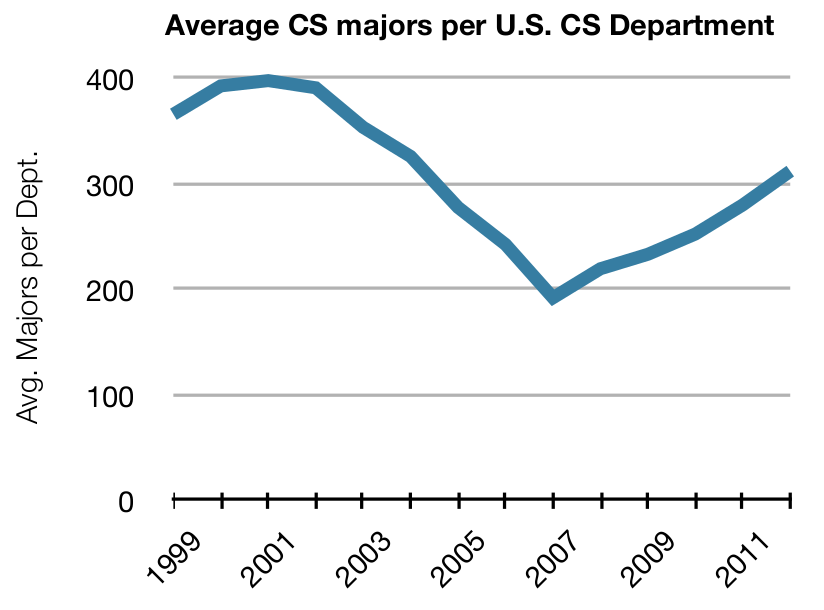
\includegraphics[width=0.5\textwidth]{figs/zweben-cs-majors.png}
    \caption{From Zweben, 2011.}
  \end{figure}
\end{frame}


\begin{frame}{Departmental Evaluation}

  Evaluating a department on its conceptual coverage involves\ldots
  \vfill
  \onslide<+->
  \begin{description}[<+- | alert@+>]
    \item[Relative Standing] comparing against other, similar departments
    \item[Absolute Performance] benchmark against standardized expectations
      (published by the ACM)
  \end{description}
  \vfill
  \uncover<+->{Both of these require data about the topics covered in a
    course.}

\end{frame}


\begin{frame}{Available Data}
  \begin{block}{What we've got:}
    \onslide<+->
    \begin{enumerate}[<+- | alert@+>]
      \item Widely available university course description data.
      \item Descriptions detail what concepts are taught in a course.
      \item \textbf{Human-readable} descriptions require manual inspection.
    \end{enumerate}
  \end{block}

  \vfill

  \uncover<5->{\begin{block}{So what to do?}\end{block}}

\end{frame}


\begin{frame}{Research Goal}

  \vfill
  Through the application of probabilistic machine learning methods,
  specifically LDA topic modeling, a corpus of unstructured course
  descriptions can be digested and mined for topics. In this scenario,
  each topic represents a core concept covered by the courses.
  \vfill
  A research framework will be constructed to read data from the
  Internet, digest into a common internal format, pipeline into an LDA
  topic model, and ultimately visualize in an interactive manner.
  \vfill
  Ultimately the automatically discovered topics can be used in end-user
  university evaluation processes.
  \vfill
\end{frame}


\begin{frame}{Research Goal}

  \begin{block}{In other words}
    Build a tool that automatically\ldots
    \onslide<+->
    \begin{itemize}[<+- | alert@+>]
      \item ingests large collection of course descriptions
      \item infers topics from course descriptions
      \item computes comparisons between departments
      \item evaluates departments on their concepts
    \end{itemize}
  \end{block}

\end{frame}


\section{Background}


\begin{frame}{Topic Modeling}

  \begin{block}{Topic Modeling}
    Attempts to discover the abstract \alert{topics} of a dataset.
  \end{block}

  \begin{block}{Topics}
    A \alert{topic} is a frequency distribution over terms, roughly
    representing a concept taught in a course.
  \end{block}
\end{frame}


\begin{frame}{Latent Dirichlet Allocation}
  \begin{block}{Overview}
    \alert{Latent Dirichlet Allocation (LDA)} is a form of \emph{Latent
    Variable Modeling} that can infer topics from within a document.
    \vfill
    LDA takes a generative approach to latent variable modeling, assuming
    the topics occur in some proportion within each document.
  \end{block}
\end{frame}


\section{Data}


\begin{frame}{University Dataset}
  \begin{table}
    \begin{tabular}{lcl}
      \toprule
      University & Course Count & Web \\
      \midrule
      American University & 32 & \href{http://american.edu}{american.edu} \\
      George Mason University & 145 & \href{http://gmu.edu}{gmu.edu} \\
      Kansas State University & 83 & \href{http://ksu.edu}{ksu.edu} \\
      Louisiana State University & 59 & \href{http://lsu.edu}{lsu.edu} \\
      Portland State University & 190 & \href{http://pdx.edu}{pdx.edu} \\
      Rensselaer Polytechnic Institute & 61 & \href{http://rpi.edu}{rpi.edu} \\
      University of South Carolina & 64 & \href{http://sc.edu}{sc.edu} \\
      Stanford University & 69 & \href{http://stanford.edu}{stanford.edu} \\
      University of Utah & 142 & \href{http://utah.edu}{utah.edu} \\
      University of Tennessee, Knoxville & 29 & \href{http://utk.edu}{utk.edu} \\
      \midrule
      ACM Exemplar Courses & 68 & --- \\
      \bottomrule
    \end{tabular}
    \caption{University course descriptions}
  \end{table}
\end{frame}


\begin{frame}{Sample Course Descriptions}
  \begin{block}{Raw Course Description}
    Capstone course focusing on design and successful implementation of
    major software project, encompassing broad spectrum of knowledge and
    skills, developed by team of students. Requires final exhibition to
    faculty-industry panel.
  \end{block}

  \begin{block}{Cleaned course description}
    capston focus design success implement major softwar project encompass
    broad spectrum knowledg skill develop team student requir final exhibit
    faculti industri panel
  \end{block}
\end{frame}


\section{Trajectory}


\begin{frame}{Trajectory}
  \textbf{Trajectory} is a tool that automatically ingests course
  description data from the Internet and presents an accessible interface
  for departmental evaluation.

  \begin{table}
    \begin{tabular}{ll}
      \toprule
      Lines of Python & 3193 \\
      Lines of Java & 631 \\
      Lines of HTML/CSS/JS & 1828 \\
      Lines of JSON & 3219 \\
      Lines of Bash & 165 \\
      \midrule
      Size on disk & 6.7M \\
      \bottomrule
    \end{tabular}
    \caption{Code statistics}
  \end{table}

\end{frame}


\begin{frame}
  \frametitle{Trajectory}
  Four primary modules:

  \begin{description}
    \item[Scrape] web-scrape online university catalogs
    \item[Import/Export] pass structured data between Learn and Scrape
    \item[Learn] estimate LDA topic model on data
    \item[Web] visualization tool
  \end{description}

  Underneath the entire system is a structured relational database layer.
\end{frame}


\begin{frame}
  \frametitle{Trajectory / Web}
  \begin{description}
    \item[Browse] collected data by university or department
    \item[Understand] courses through inferred topics
    \item[Analyze] conceptual overlap in prerequisite chains
    \item[Compare] departments based on conceptual composition
    \item[Evaluate] departments against ACM benchmarks
  \end{description}
\end{frame}


%\plain{Live Demo \\\small wish me luck!}
\plain{(Not So) Live Demo}


\begin{frame}
  \frametitle{Disclaimer}
  Images have been modified to fit in this presentation.
  \vfill
  Visit \url{trajectory.rouly.net} on your smart device to follow along.
\end{frame}

\section{Browse}

\begin{frame}
  \frametitle{Trajectory / Web / Browse}
  \begin{figure}
    \centering
    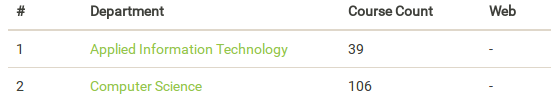
\includegraphics[width=0.95\textwidth]{figs/shots/departments.png}
    \caption{Browse a university's departments.}
  \end{figure}
\end{frame}

\begin{frame}
  \frametitle{Trajectory / Web / Browse}
  \begin{figure}
    \centering
    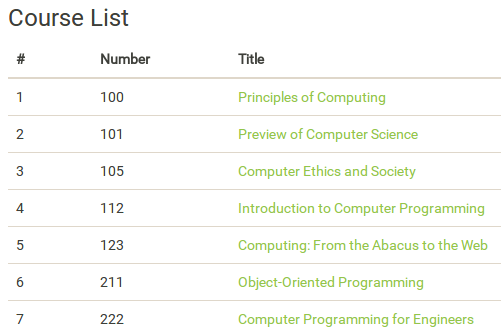
\includegraphics[width=0.75\textwidth]{figs/shots/courses.png}
    \caption{Browse a department's courses.}
  \end{figure}
\end{frame}

\section{Understand}

\begin{frame}
  \frametitle{Trajectory / Web / Understand}
  \begin{figure}
    \centering
    
\includegraphics[width=0.95\textwidth]{figs/shots/course_detail.png}
    \caption{View a course's inferred topics.}
  \end{figure}
\end{frame}

\begin{frame}
  \frametitle{Trajectory / Web / Understand}
  \begin{figure}
    \centering
    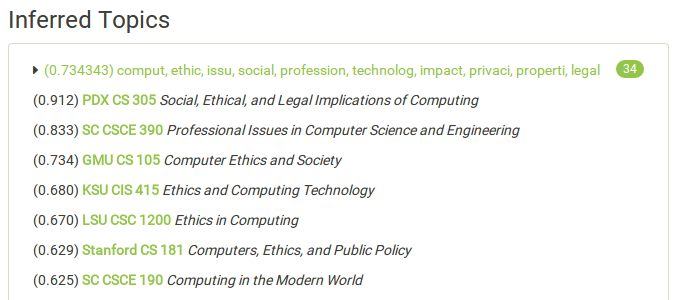
\includegraphics[width=0.95\textwidth]{figs/shots/related_ethics.png}
    \caption{View related courses.}
  \end{figure}
\end{frame}

\begin{frame}
  \frametitle{Trajectory / Web / Understand}
  \begin{figure}
    \centering
    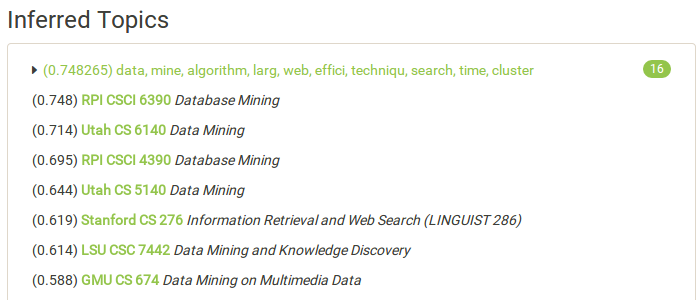
\includegraphics[width=0.95\textwidth]{figs/shots/related_data_mining.png}
    \caption{View related courses.}
  \end{figure}
\end{frame}

\begin{frame}
  \frametitle{Trajectory / Web / Understand}
  \begin{figure}
    \centering
    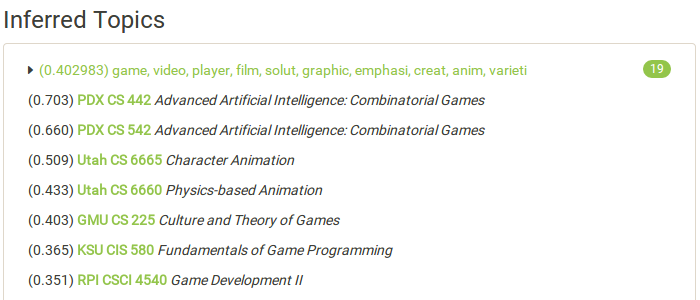
\includegraphics[width=0.95\textwidth]{figs/shots/related_game_design.png}
    \caption{View related courses.}
  \end{figure}
\end{frame}

\section{Analyze}

\begin{frame}
  \frametitle{Trajectory / Web / Analyze}
  \begin{figure}
    \centering
    \includegraphics[width=0.95\textwidth]{figs/shots/prereq_tree.png}
    \caption{Course prerequisite tree.}
  \end{figure}
\end{frame}

\section{Compare}

\begin{frame}
  \frametitle{Trajectory / Web / Compare}
  \begin{figure}
    \centering
    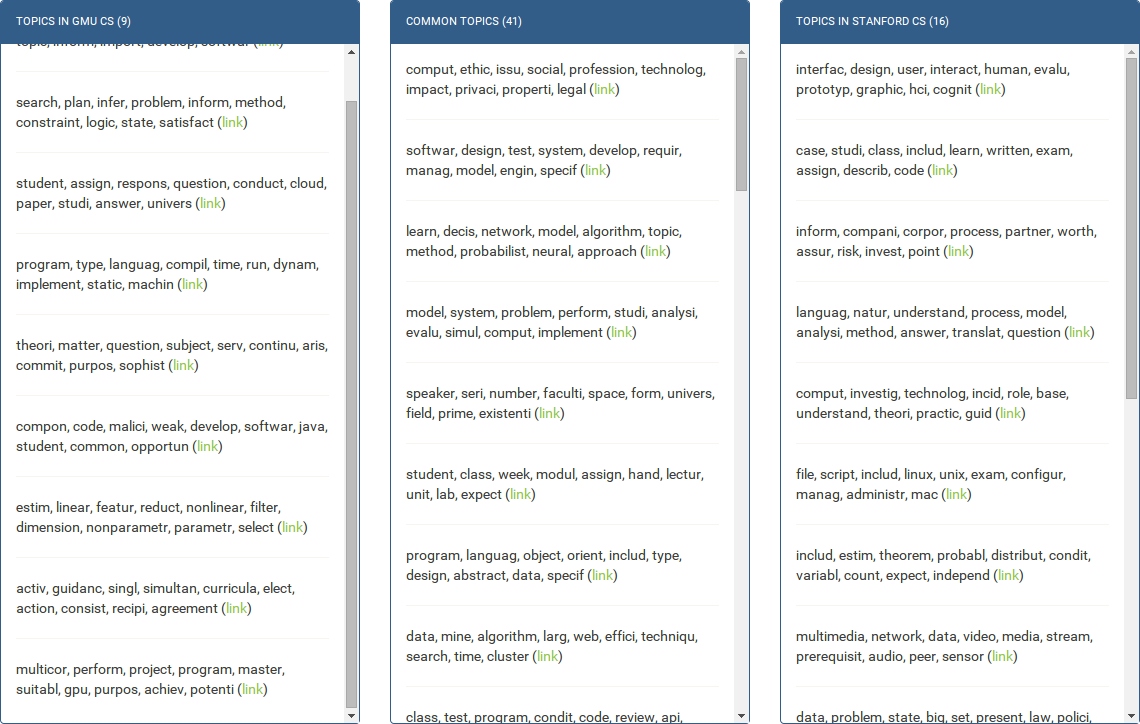
\includegraphics[width=0.95\textwidth]{figs/shots/compare.png}
    \caption{Compare departmental concept coverage.}
  \end{figure}
\end{frame}

\begin{frame}
  \frametitle{Trajectory / Web / Compare}
  \begin{figure}
    \centering
    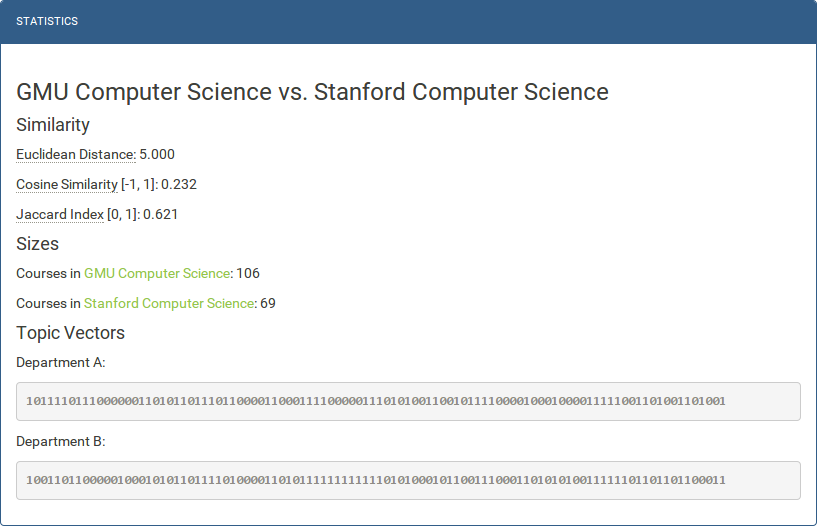
\includegraphics[width=0.95\textwidth]{figs/shots/stats.png}
    \caption{Quick departmental comparison.}
  \end{figure}
\end{frame}

\section{Evaluate}

\begin{frame}
  \frametitle{Trajectory / Web / Evaluate}
  \begin{figure}
    \centering
    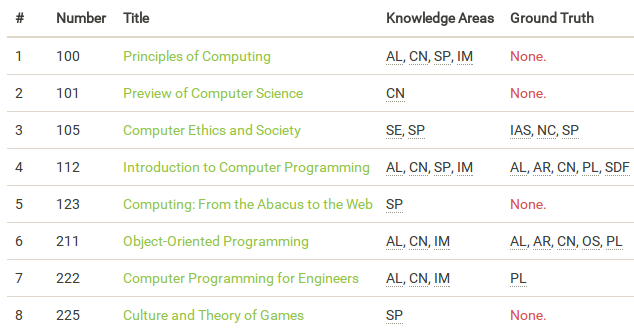
\includegraphics[width=0.95\textwidth]{figs/shots/evaluation.png}
    \caption{Evaluate department against Knowledge Areas.}
  \end{figure}
\end{frame}


\section{Wrap up}


\begin{frame}
  \frametitle{Future Goals}
  \begin{itemize}
    \item Learning Outcomes meta-analysis
    \item Alternative methods
    \item Topic summarization
    \item Extension to workforce preparedness
    \item Smart web scraping
  \end{itemize}
\end{frame}


\begin{frame}{Summary}

  Try out \textbf{Trajectory} online at

  \begin{center}\url{trajectory.rouly.net}\end{center}

  Get the source of this presentation and the \textbf{Trajectory} project
  at

  \begin{center}\url{github.com/jrouly/trajectory}\end{center}

  \vfill

  \textbf{Trajectory} is licensed under the
  \href{http://www.apache.org/licenses/LICENSE-2.0}{Apache version 2.0
  license}.

\end{frame}


\begin{frame}{Credits}
  Co-authors:
  \begin{itemize}
    \item Huzefa Rangwala
    \item Aditya Johri
  \end{itemize}

  Presentation theme:
  \begin{itemize}\item\url{github.com/matze/mtheme}\end{itemize}
\end{frame}


\begin{frame}{Primary Sources}
  \begin{itemize}
    \item D. M. Blei, A. Y. Ng, and M. I. Jordan. Latent Dirichlet Allocation.
      \emph{J. Mach. Learn. Res.}, 3:993–1022, Mar. 2003.
    \item ACM/IEEE-CS Joint Task Force on Computing
      Curricula. Computer science curricula 2013. Technical
      report, ACM Press and IEEE Computer Society
      Press, December 2013.
    \item S. Zweben. Computing degree and enrollment trends.
      Technical report, Computing Research Association,
      2011.
  \end{itemize}
\end{frame}


\plain{Questions?}


\end{document}
